\begin{figure}[h]
    \centering
    \setlength{\tikzunit}{\textwidth/16}
    \begin{tikzpicture}[scale=1, x=\tikzunit,y=\tikzunit]
        \node(0,0) {};
        \draw( 4.0, 4.0) node{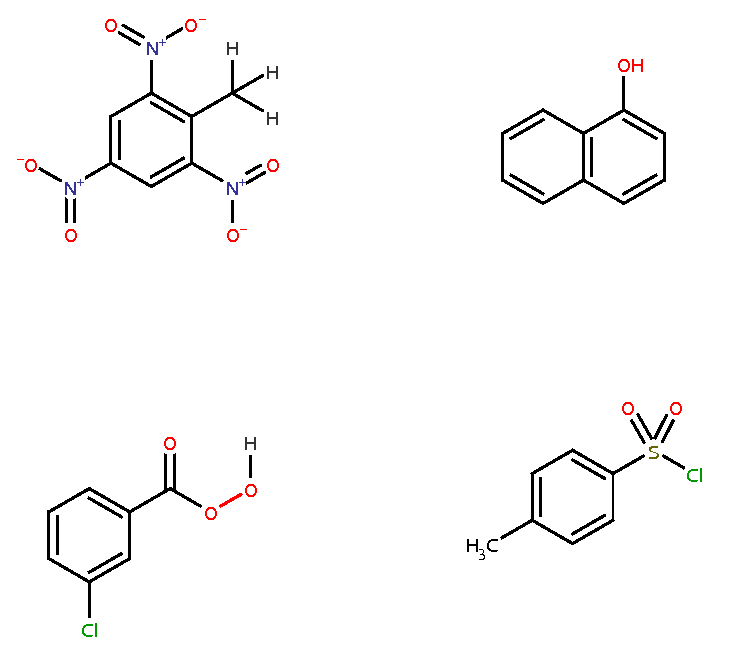
\includegraphics[width=7\tikzunit]{4struct.eps}};
        \draw(-4.0, 4.0) node{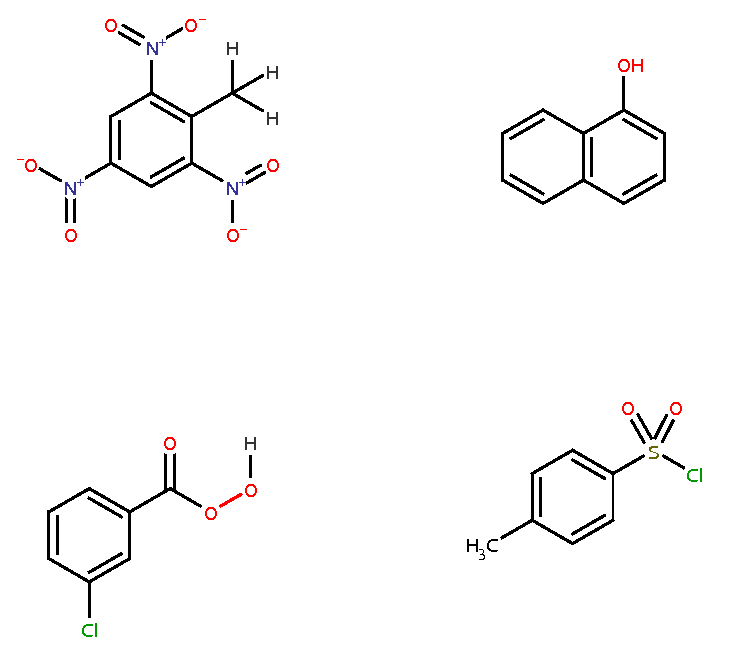
\includegraphics[width=7\tikzunit]{4struct.eps}};
        \draw( 4.0,-4.0) node{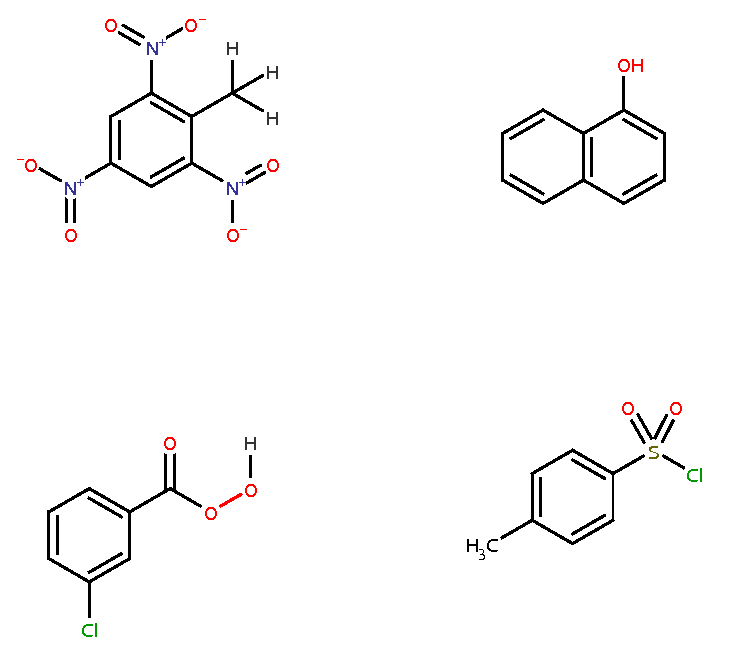
\includegraphics[width=7\tikzunit]{4struct.eps}};
        \draw(-4.0,-4.0) node{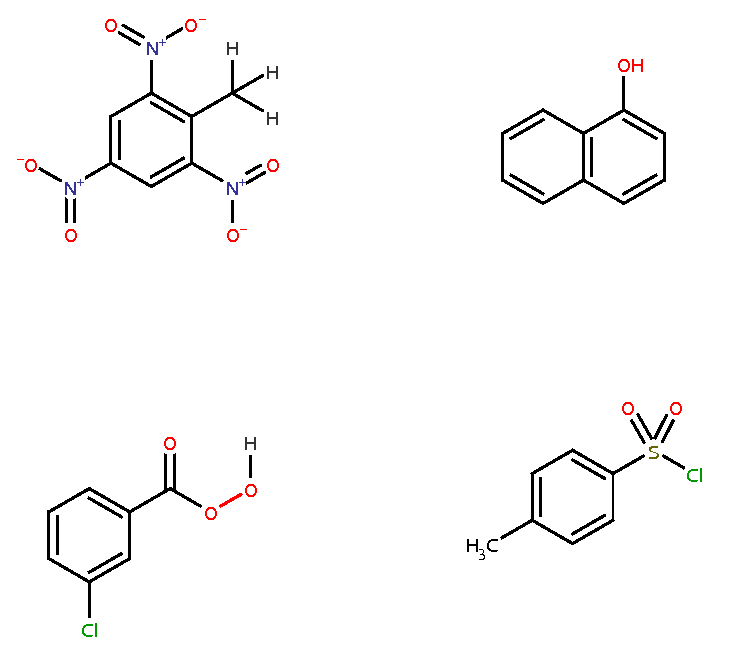
\includegraphics[width=7\tikzunit]{4struct.eps}};
        \draw(-7.5, 7.5) node{\textbf{a)}};
        \draw( 0.5, 7.5) node{\textbf{b)}};
        \draw(-7.5,-0.5) node{\textbf{c)}};
        \draw( 0.5,-0.5) node{\textbf{d)}};
        \draw[step= .5,color=gray,thin,dashed]( 0, 0) grid ( 8, 8);
        \draw[step=1.0,color=gray]            ( 0, 0) grid ( 8, 8);
        \draw[step=4.0,color=black]           ( 0, 0) grid ( 8, 8);
        \draw[step= .5,color=gray,thin,dashed](-8,-8) grid ( 0, 0);
        \draw[step=1.0,color=gray]            (-8,-8) grid ( 0, 0);
        \draw[step=4.0,color=black]           (-8,-8) grid ( 0, 0);
%        \draw(-0.5, 4.0) node{$\Longrightarrow$};
%        \draw(-8.5,-4.0) node{$\Longrightarrow$};
%        \draw( 0.5,-4.0) node{$\Longrightarrow$};
        \draw (-6.1, -3.5) node{TNT};
        \draw (-6.1, -7.5) node{\compx{1}};
        \draw (-2.0, -3.5) node{Naphtol};
        \draw (-2.0, -7.5) node{\compx{2}};
        \draw ( 1.9, -3.5) node{TNT};
        \draw ( 1.9, -7.5) node{\compx{1}};
        \draw ( 6.1, -3.5) node{Naphtol};
        \draw ( 6.1, -7.5) node{\compx{2}};
    \end{tikzpicture}
    \caption{The workflow of placing the text on top of the figure. The 4 steps
    of producing good graphics are shown from the top left corner. The initial
    figure \textbf{a)} did not contain names and the grid was added
    at \textbf{b)} to help determine the position of the labels, which where
    placed at \textbf{c)} and then the grid was removed at \textbf{d)}. NB this
    ilustration was done also using the very same TikZ package.}
    \label{fig:struct1-1} 
\end{figure}
